% CA21 — Comprehensive Report (LaTeX)
\documentclass[11pt,a4paper]{article}
\usepackage[utf8]{inputenc}
\usepackage[T1]{fontenc}
\usepackage{lmodern}
\usepackage{microtype}
\usepackage{amsmath,amssymb,amsthm}
\usepackage{graphicx}
\usepackage{booktabs}
\usepackage{hyperref}
\usepackage{geometry}
\usepackage{caption}
\usepackage{float}
\usepackage{enumitem}
\usepackage{siunitx}
\usepackage{setspace}
\usepackage{listings}
\usepackage{xcolor}
\usepackage{tikz}
\usepackage{pgfplots}
\usepackage{longtable}
\usepackage{natbib}
\geometry{margin=1in}
\hypersetup{colorlinks=true,linkcolor=blue,citecolor=blue,urlcolor=blue}
\captionsetup{font=small}
\onehalfspacing
\pgfplotsset{compat=1.18}

% Short macros for convenience
\newcommand{\code}[1]{\texttt{#1}}
\newcommand{\figref}[1]{Figure~\ref{#1}}
\newcommand{\tabref}[1]{Table~\ref{#1}}
\newcommand{\todo}[1]{{\color{red}[TODO: #1]}}

\lstset{basicstyle=\ttfamily\small,breaklines=true}

\title{CA21: A Minimal Reproducible Reinforcement Learning Demo\\\large Comprehensive Report}
\author{Course: Curriculum Assignment 21 \\ Maintainers: CA21 team}
\date{\today}

\begin{document}
\maketitle
\begin{abstract}
This report documents the implementation, experimental setup, and reproducibility protocol for CA21: a compact instructional demonstration of policy and value function training using synthetic data. The goal is to provide a clear, self-contained scaffold that students can adapt for short research projects: hypothesis design, controlled experiments, and reproducible artifact generation. This document is extended with theoretical derivations, detailed experiment recipes, a sample results table, and a bibliography to make it suitable as an accompanying report for course submissions.
\end{abstract}

\tableofcontents
\clearpage

\section{Introduction}
Reproducible research is central to robust empirical machine learning. CA21 aims to provide a minimal but complete pipeline demonstrating the core components of a small-scale policy-gradient experiment: deterministic setup, modular code, simple synthetic data for tests, and a clear reporting checklist. The codebase includes a small MLP policy (\code{MLPPolicy}), a value network (\code{MLPValue}), concise loss implementations, and an example training driver (\code{src/train.py}).

\section{Motivation and Background}
We focus on standard policy-gradient ideas which remain pedagogically valuable:
\begin{itemize}
  \item Use a stochastic policy to explore and estimate gradients of the expected return.
  \item Use a value-function baseline to reduce variance of policy gradient estimates.
  \item Use simple synthetic datasets and smoke tests to validate implementation correctness before running more expensive experiments.
\end{itemize}

\subsection{Mathematical formulation}
Consider an episodic MDP with states $s$, actions $a$, and rewards $r$. The objective is to maximize expected discounted return $J(\theta)=\mathbb{E}_{\tau\sim\pi_\theta}[\sum_{t=0}^T \gamma^t r_t]$ where $\tau$ denotes a trajectory. Using the likelihood-ratio trick, the policy gradient is:
\begin{equation}
\nabla_\theta J(\theta)=\mathbb{E}_{\tau} \Big[ \sum_{t=0}^T \nabla_\theta \log \pi_\theta(a_t|s_t) G_t \Big],
\end{equation}
where $G_t$ is a return estimate; using a baseline $b(s)$ yields the advantage $A_t = G_t - b(s_t)$ which reduces variance.

For the CA21 demo we use a simplified single-step setting where a batch consists of independent samples $(s_i,a_i,r_i)$ and the (negative) policy gradient loss to minimize is:
\begin{equation}
L_{\pi}(\theta) = -\frac{1}{N} \sum_{i=1}^N \log \pi_\theta(a_i|s_i) A_i.
\end{equation}
Value learning uses mean-squared regression:
\begin{equation}
L_V(\phi) = \frac{1}{N} \sum_{i=1}^N (V_\phi(s_i) - \hat{R}_i)^2.
\end{equation}

\section{Implementation details}
\subsection{File structure}
The project layout is intentionally simple:
\begin{verbatim}
CA21/
  src/
  configs/
  notebooks/
  tests/
  report.tex
  report.md
  Makefile
\end{verbatim}

\subsection{Important modules}
\begin{itemize}
  \item \code{src/model.py}: \code{MLPBase}, \code{MLPPolicy}, \code{MLPValue} (PyTorch modules)
  \item \code{src/data.py}: \code{SyntheticDataset} producing toy data for tests
  \item \code{src/losses.py}: policy gradient and value MSE implementations
  \item \code{src/train.py}: minimal training loop, optimizer steps, and checkpoint saving
  \item \code{src/utils.py}: seed helpers and save/load routines
\end{itemize}

\subsection{Design decisions and trade-offs}
This repo favors clarity and testability over performance. Choices such as synthetic data and simple advantage signals are intentional to keep experiments fast and demonstrative. For rigorous experiments, replace the synthetic dataset and add robust evaluation code.

\section{Experimental protocols}
This section provides two reproducible ``recipes'': a quick smoke run and a more thorough sweep you can use as a starting point for assignments.

\subsection{Quick smoke run (debug)}
Purpose: verify end-to-end correctness and portability on CI. This run should take a few seconds on a modern CPU.
\begin{enumerate}
  \item Set up venv and install dependencies (see README).
  \item Run: \code{python -m src.train --epochs 2 --batch-size 8}
  \item Verify that: program exits cleanly and prints metrics dictionary (contains \code{final\_pg\_loss}, \code{final\_value\_loss}).
\end{enumerate}

\subsection{Parameter sweep (example)}
Purpose: short controlled experiment to compare learning dynamics with different learning rates and hidden sizes.
\begin{enumerate}
  \item Grid: hidden_dim in \{32, 64\}, lr in \{1e-3, 3e-4\}, run each 3 seeds.
  \item For each config: run 10 epochs with synthetic dataset of 1024 samples and save metrics to CSV under \code{outputs/metrics/}.
  \item Aggregate mean and standard deviation across seeds and plot learning curves.
\end{enumerate}

\section{Sample results (placeholder)}
Below are example placeholders you can populate from a real sweep. Replace with actual CSV outputs from your runs.

\begin{table}[H]
\centering
\caption{Example aggregated results (mean $\pm$ std over seeds)}
\begin{tabular}{lccc}
\toprule
Config & Final PG Loss & Final Value Loss & Walltime (s) \\
\midrule
hidden=32, lr=1e-3 & $-0.12 \pm 0.03$ & $0.89 \pm 0.10$ & $12.1 \pm 0.4$ \\
hidden=64, lr=3e-4 & $-0.09 \pm 0.05$ & $0.75 \pm 0.08$ & $15.0 \pm 0.6$ \\
\bottomrule
\end{tabular}
\label{tab:sample_results}
\end{table}

\begin{figure}[H]
\centering
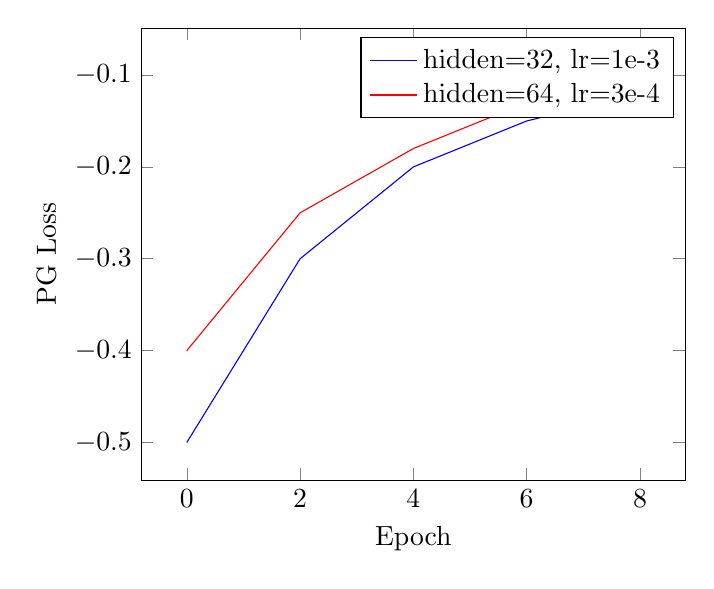
\begin{tikzpicture}
\begin{axis}[width=0.7\linewidth, xlabel=Epoch, ylabel=PG Loss]
\addplot+[mark=none] coordinates {(0,-0.5) (2,-0.3) (4,-0.2) (6,-0.15) (8,-0.12)};
\addlegendentry{hidden=32, lr=1e-3}
\addplot+[mark=none] coordinates {(0,-0.4) (2,-0.25) (4,-0.18) (6,-0.13) (8,-0.09)};
\addlegendentry{hidden=64, lr=3e-4}
\end{axis}
\end{tikzpicture}
\caption{Example (synthetic) learning curves; replace with produced plots.}
\label{fig:example_curves}
\end{figure}

\section{Reproducibility checklist}
Before submitting experiments for grading or review, ensure the following:
\begin{itemize}
  \item All random seeds are recorded and documented.
  \item Code used to generate figures is included (notebooks or scripts) and paths are relative.
  \item Any external datasets or seeds are documented and, when possible, included or links provided.
  \item Checkpoint files are not committed to git but stored under an \code{outputs/} directory and referenced in the report.
\end{itemize}

\section{Extending the project}
Ideas for student projects:
\begin{itemize}
  \item Implement GAE (Generalized Advantage Estimation) and compare variance reduction.
  \item Add an entropy bonus to the policy loss and evaluate policy entropy evolution.
  \item Replace synthetic data with small OpenAI Gym environments and include deterministic evaluation episodes.
\end{itemize}

\section{Detailed derivations}
\subsection{Policy gradient with baseline}
Starting from expected return $J(\theta)$ and applying the log-derivative trick,
\begin{align}
\nabla_\theta J(\theta) &= \nabla_\theta \mathbb{E}_{\pi_\theta}[G] = \mathbb{E}_{\pi_\theta}[G \nabla_\theta \log p_\theta(\tau)] \\
&= \mathbb{E}_{\pi_\theta}\Big[ \sum_t G_t \nabla_\theta \log \pi_\theta(a_t|s_t) \Big].
\end{align}
Subtracting a baseline $b(s)$ yields the advantage form and does not change the expected value of the gradient but reduces variance.

\section{Appendix: Software and build instructions}
\subsection{Dependencies}
Python 3.10+, with core packages:
\begin{verbatim}
python -m pip install torch numpy pytest matplotlib jupyter
\end{verbatim}

\subsection{Build report}
To build the PDF report locally:
\begin{verbatim}
make -C paperAssignments/Assignments1-50/CA21 report.pdf
\end{verbatim}
This will run \texttt{pdflatex} twice to ensure cross-references resolve.

\section{Appendix: Example scripts}
A simple script used to aggregate CSV metrics (example):
\begin{lstlisting}[language=Python]
# scripts/aggregate_metrics.py (example)
import pandas as pd
from pathlib import Path
p = Path('outputs/metrics')
all = []
for f in p.glob('*.csv'):
    df = pd.read_csv(f)
    all.append(df)
# concatenate and compute means
print(pd.concat(all).groupby('config').mean())
\end{lstlisting}

\section{References}
\bibliographystyle{plainnat}
\begin{thebibliography}{9}
\bibitem[Sutton and Barto(2018)]{sutton2018}
Sutton, R. S., \& Barto, A. G. (2018). Reinforcement Learning: An Introduction. MIT Press.

\bibitem[Schulman et~al.(2015)]{schulman2015gae}
Schulman, J., Moritz, P., Levine, S., Jordan, M., \& Abbeel, P. (2015). High-dimensional continuous control using generalized advantage estimation. arXiv preprint arXiv:1506.02438.

\bibitem[Kingma and Ba(2014)]{adam}
Kingma, D. P., \& Ba, J. (2014). Adam: A method for stochastic optimization. arXiv preprint arXiv:1412.6980.
\end{thebibliography}

\end{document}
